\documentclass[letterpaper]{article}
\usepackage{import}{\tiny }
\usepackage{standalone}
\usepackage[english]{babel}
\usepackage[a4paper]{geometry}
\usepackage[utf8]{inputenc}
\usepackage{float}
\usepackage{amsmath}
\usepackage{amssymb}
\usepackage{amsthm}
%\usepackage{cool} %seems cool. has bugs. conflicts with own derivative commands (below)
\usepackage{enumitem}
\usepackage{fancyhdr}
\usepackage{multirow}
\usepackage{booktabs}
\usepackage{subfiles}
\usepackage{siunitx}
\usepackage{graphicx}
\usepackage{caption}
\usepackage{subcaption}
\usepackage{hyperref}
\usepackage{appendix}
\usepackage{rotating}
\pagestyle{fancy}

%Packages and settings for code formatting
\usepackage{color}
\definecolor{code_keywords}   {rgb}{0,0,0} %blue={0.13,0.13,0.75}
\definecolor{code_comments}   {rgb}{0.17,0.57,0.17}
\definecolor{code_linenumbers}{rgb}{0.5,0.5,0.5}
\definecolor{code_strings}    {rgb}{0,0,0} %red={0.5,0,0}
\usepackage{listings}
\lstset{
	language		 = Matlab,
	basicstyle		 = \footnotesize,
	commentstyle	 = \color{code_comments},
	keywordstyle	 = \bfseries\color{code_keywords},
	stringstyle		 = \color{code_strings},
	numberstyle		 = \tiny\color{code_linenumbers},
	frame			 = none,
	keepspaces		 = true,
	numbers			 = left,
	numbersep		 = 5pt,
	showspaces		 = false,
	showstringspaces = false,
	showtabs		 = false,
	stepnumber		 = 1,
	tabsize			 = 4,
}


\lfoot{} % Controls the left corner of the footer
\cfoot{} % Controls the center of the footer
\rfoot{page~\thepage} % Controls the right corner of the footer
\renewcommand{\headrulewidth}{0.4pt}
\renewcommand{\footrulewidth}{0.4pt}

%Specify table columns' width
\newcolumntype{L}[1]{>{\raggedright\arraybackslash}p{#1}}
\newcolumntype{C}[1]{>{\centering\arraybackslash}p{#1}}
\newcolumntype{R}[1]{>{\raggedleft\arraybackslash}p{#1}}


\newcommand{\todo}[1]{\textcolor{red}{\textbf{[TODO]}~#1}}

\newcommand{\imp}{\Rightarrow} %mathematical "implies"
\newcommand{\Imp}{\quad\imp\quad} %...with spacing


\author{Giovanni Bologni (4757386) and Wouther Bons (4092716)}
\date{\today}
\title{EE4389\\Modeling and Data Analysis in Complex Networks\\Assignment}
\lhead{EE4389 Complex Networks Assignment} % Controls the left corner of the header
\chead{} % Controls the center of the header
%\rhead{Giovanni Bologni and Wouther Bons} % Controls the right corner of the header

\begin{document}

\maketitle

\subsection*{Introduction}
When measurements are performed on a network, the resulting dataset can be analysed to quantify properties of the underlying network. In this assignment a dataset of face-to-face contact data of highschool students\footnote{R. Mastrandrea, J. Fournet, A. Barrat, Contact patterns in a high school: a comparison between data collected using wearable sensors, contact diaries and friendship surveys. PLoS ONE 10(9): e0136497 (2015)} is analysed.

This data not only includes contact information at a certain time, but also how contact changes over time; every measurement specifies which two students have had contact and at which time this occured. Students will be modeled as nodes in a graph and contact between students as edges. Each edge will also be labeled with the timestamp at which the contact it represents was made.

To begin with, this data will be aggregated over all time to analyse the topology of the resulting aggregated network. Secondly, the time of measurement will be taken into consideration. Several metrics will be used to analyse which nodes are most influential when information spreads across this temporal network. Lastly, temporal features of the network will be altered to inspect their influence on the information spreading process.

\subsection*{Part A: Topological features of the aggregated network}
\label{sec:partA}

All measured topological features are summarized in table \ref{tab:topological_features}.

%\setlength\LTleft{0pt} % left-align rather than center-set the longtable
\begin{table}[ht!]
	\centering
	\begin{tabular}{@{} L{10em} L{5em} R{2.5em} @{} L{2.5em} @{}}
	\toprule
	\textbf{Topological feature} & ~ & \multicolumn{2}{r}{\textbf{Value}}\\
	\midrule
	Number of nodes& N & 327& \\
	Number of links& L & 5818& \\ 
	Link density& p  & 0&.1092 \\ 
	Average degree& $E[D]$  & 35&.58\\
	Degree variance& $Var[D]$ & 182&.2 \\
	Degree assortativity& $\rho_D$ & 0&.03318\\
	Clustering coefficient& C & 0&.5035\\
	Average hopcount& $E[H]$ & 2&.159\\
	Diameter& $H_{max}$ & 4& \\
	Spectral radius& $\lambda_1$ & 41&.23\\
	Algebraic connectivity& $\mu_{N-1}$ & 1&.93\\
	\bottomrule
	\end{tabular}
	\caption{List of all topological features of the aggregated network that were examined. For details on calculations and interpretations see part \ref{sec:partA}.}
	\label{tab:topological_features}
\end{table}

The aggregated graph \(G\) is constructed by connecting any two nodes by an (unweighted) edge if the nodes make contact with eachother at least once in the \(T=7375\) timesteps available.

\(G\) has \(N=327\) nodes and \(L=5818\) links. The link density is computed as
\begin{align*}
p = \frac{E[L]}{L_{max}} = \frac{L}{N(N-1)/2} = 0.1092
\end{align*}

Several metrics inspect the degree of nodes in the network, of which an insightful one is the degree distribution (fig.~\ref{fig:degree_distribution_aggregated}). It can be seen that this distribution resembles a Poisson distribution. This suggests that an Erdös-Renyi (ER) graph model would be well suited to model the face-to-face contact network. In contrast, a scale-free graph model would be a bad choice of model because scale-free graphs show a linear distribution when viewed on a log-log scale and this is absolutely not the case (fig.~\ref{fig:degree_distribution_loglog}).

The average and variance of the degree are \(E[D]=35.58\) and \(Var[D]=182.2\), respectively. The degree assortativity (\(\rho_D=0.03318\)) is defined as the (linear) correlation coefficient between the degrees of nodes, so a value of almost zero means the degrees of nodes are not correlated at all. This means that the creation of new links is not influenced by existing links; another argument for using the ER graph model, where edges are created with independent probabilities (and are therefore uncorrelated).

\begin{figure}
    \centering
    \begin{subfigure}[b]{0.45\textwidth}
        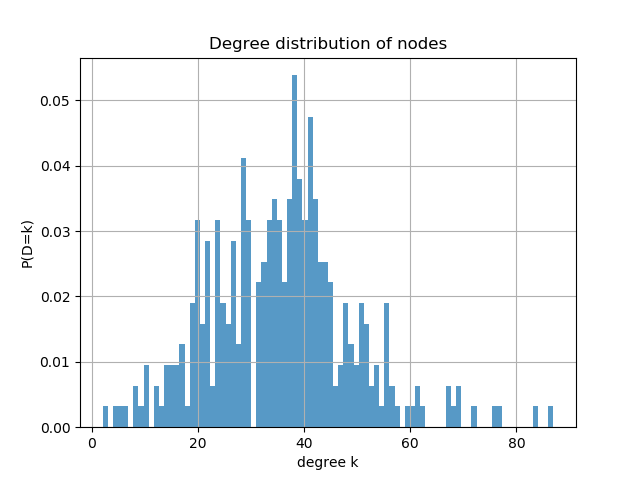
\includegraphics[width=\textwidth]{img/degree_distribution.png}
        \caption{Linear scale}
	    \label{fig:degree_distribution_linlin}
    \end{subfigure}
    ~ % spacing
    \begin{subfigure}[b]{0.45\textwidth}
        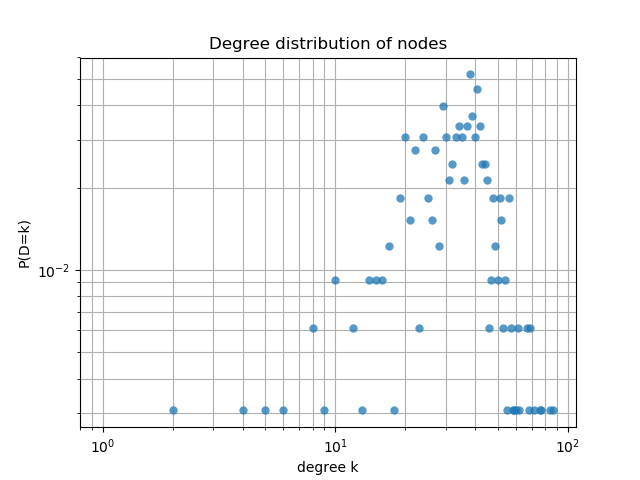
\includegraphics[width=\textwidth]{img/degree_distribution_loglog.png}
        \caption{Log scale}
	    \label{fig:degree_distribution_loglog}
    \end{subfigure}
    \caption{Degree distribution of nodes in the aggregated graph.}
    \label{fig:degree_distribution_aggregated}
\end{figure}

Furthermore, it is interesting to check whether the network exhibits the small-world property, i.e. nodes are not very clustered but can still reach other nodes in relatively few hops. Using the clustering coefficient (\(C=0.5035\)) and average hopcount (\(E[H]=2.159\)) normalized by that of the regular graph results in the following metrics: \todo{suspicious that they're larger than one...}
\begin{align*}
C/C(0) = 4.681\\
E[H]/E[H](0) = 1.132
\end{align*}
Because the (normalized) clustering coefficient is several times higher than the average hopcount, the network exhibits the small-world property. \todo{C\(>\)E[H] shows from the graph on the slides, but I thought the clustering had to be lower, not higher?!}

\todo{L proportional to log N for small-world networks (plot over time) better test for small-world property?}

Comparing the average hopcount (\(E[H]=2.159\)) with the diameter of the graph (\(H_{max}=4\)) we see that there is not a lot of variance in hopcounts of shortest paths between nodes; the diameter (the worst-case hopcount of shortest paths) is close to the graph's efficiency (the average hopcount). This again points to the small-world property.

Lastly, some spectral metrics of the aggregated graph are considered. The spectral radius is calculated as the largest eigenvalue of the adjacency matrix \(\lambda_1=41.23\). The algebraic connectivity is the second smallest eigenvalue of not the adjacency but the Laplacian matrix, \(a=\mu_{N-1}=1.930\). \todo{is this a lot or not? perhaps compare with upper bound 1/nD where n is nodes in complete graph?}


\subsection*{Part B: Information spreading on a temporal network}
%9) Taking all the N iterations into count, plot the average number of infected nodes E[I(t)] together with
%its error bar (standard deviation pV ar[I(t)]) as a function of the time step t.

As mentioned in the introduction, each edge was labeled with the timestamp at which the contact between students it represents was made. This means we can simulate the spread of information over the network over time. The information spreading process used is as follows: an infected node can infect any nodes it is in contact with (i.e. its neighbours at a specific timestamp), but these neighbours can only start infecting other nodes at the next timestamp. Infection starts with some selected seed node. This simulation is done N times; every node is a seed node once. Graphs of the number of infected nodes \(I(t)\) (e.g. fig.~\ref{fig:infections_G}) will show the average \(E[I(t)]\) as well as the standard deviation \(\sqrt{Var[I(t)]}\) over these N simulations.

One metric used to quantify how fast information spreads over the temporal network is the timestamp at which 80\% of all nodes have been infected. For every simulation the seed node and timestamp of 80\% infection is recorded. By sorting the seed nodes by their 80\% infection timestamps, the nodes are ranked according to their influence as a seed node, i.e. \(R=[R_{(1)}, R_{(2)}, ..., R_{(N)}]\). This ordering can now be used as a standard to quantify nodes' influence. Using the same process nodes can be ranked using other metrics (e.g. the degree, \(D=[D_{(1)}, D_{(2)}, ..., D_{(N)}]\)) and subsequently compared with R by checking how many nodes are in the same top-f fraction for both metrics, R and D. This is called the top-f recognition rate and is calculated as:
\begin{align*}
	r_{RD}(f) = \frac{\left|R_f \cap D_f\right|}{\left|R_f\right|}
\end{align*}

Several metrics are compared to R using this procedure. The results can be found in figure \ref{fig:rankG}. The temporal metrics were calculated as follows at each timestamp and for each node \(i\):

\begin{align*}
	TD_i &= \frac{D_i}{t^2+t}\\
	XTD_i &= 
		\begin{cases}
		\frac{D_i}{t}& \text{if node connected to new neighbours at this timestamp}\\
		0& otherwise
		\end{cases}
\end{align*}

The reasoning behind these metrics is that earlier contacts are more influential than later ones. For example, at later timestamps a significant part of contacts between nodes is a repetition of contact at an earlier timestamp. The temporal degree (TD) tries to account for this reduced nodal influence at later timestamps by weighing the degree with something inversely propertional to the timestamp. Additionally, the exclusive temporal degree (XTD) discards (i.e. zero weight) any repeated contact between nodes.

Figure \ref{fig:rankG} shows the results of these temporal metrics as well as several non-temporal ones. Because the comparison is done as a fraction the ideal metric would yield a unity recognition rate, i.e. ranking nodes' influence using that metric yields exactly the same results as ranking by 80\% infection timestamps (R). Therefore a value closer to unity in figure~\ref{fig:rankG} means a better metric. With this in mind, it is clear that both temporal metrics perform better than non-temporal ones, which is to be expected as they use more information.

It should be noted, however, that a linear recognition rate with unit slope means that using the metric to rank nodal influence performs the same as tossing a coin, e.g. if 40\% of nodes in the top-40\% match with R. From figure~\ref{fig:rankG}, this implies neither the degree, clustering coefficient nor betweenness are significantly better than random chance at predicting nodal influence.

\begin{figure}[ht!]
  \centering
   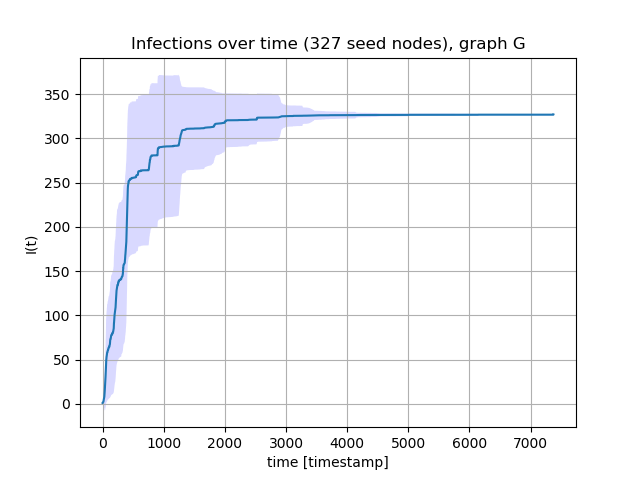
\includegraphics[width=\textwidth]{img/infections_G.png}
   \caption{The average number of infected nodes as a function of the time step, $\mathrm{E}[I(t)]$, 
 on the temporal graph $G_{data}$. The standard deviation, $\sqrt{\mathrm{Var}{[I(t)}]}$ is indicated by the shaded area.}
   \label{fig:infections_G}
\end{figure}

% question 13:
One caveat of using the top-f recognition rate is that it artifically separates nodes for which a metric has the same value. For example, consider a small graph of five nodes, where node 1 through 4 all have degree 1 and node 5 has a higher degree. The ranking nodes by degree could then be any permutation of nodes 1 through 4, followed by 5, e.g. \(D=[D_{(1)},D_{(2)},D_{(3)},D_{(4)},D_{(5)}]\) or \(D=[D_{(2)},D_{(4)},D_{(1)},D_{(3)},D_{(5)}]\). The top-f recognition rate then depend on the permutation of nodes with equal degree, while in reality the nodes perform equally well and should theoretically all four "share" first place. This effect is neglegible for very large networks but is important to take into consideration when using top-f recognition rates for smaller networks.


\begin{figure}[ht!]
  \centering
   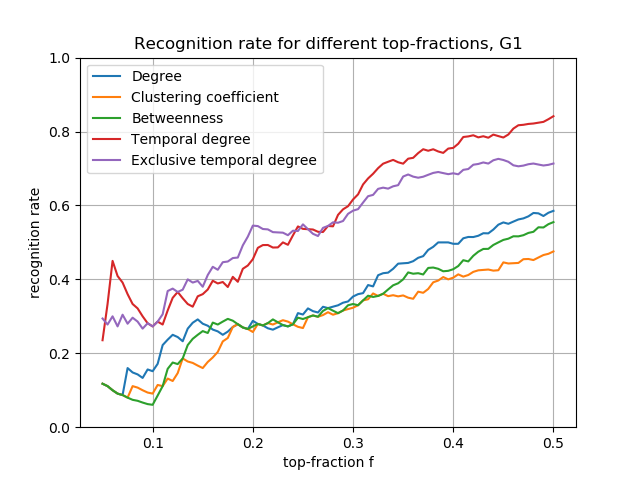
\includegraphics[width=0.8\textwidth]{img/rankG.png}
   \caption{The top $f$ recognition rate $r_{RX}(f) = \frac{ |R_f \cap X_f| }{ |R_f| }$, where $R_f$ and $X_f$ are the sets of nodes ranking in the top $f$ fraction according to their influence,  or to another metric $X(f)$, respectively. The metrics based on the temporal features are more accurate in detecting the most influential seed nodes.}
   \label{fig:rankG}
\end{figure}


\subsection*{Part C: Influence of temporal network features on information spreading}
\label{sec:partC}
% Construct the following three temporal networks. G2 is exactly the same as Gdata except that the time
%stamps describing when each temporal link (contact) appears in Gdata are randomlized in G2. In other words,
%G2 is constructed by copying all the temporal links from Gdata but their time stamps are randomly re-shuffled
%or equivalently, randomly reassigned to the temporal links. The number of contacts between each node pair is
%the same between Gdata and G2. [A time stamp vector v, whose length equals the number of contacts, can be
%randomly reshuffled to a vector v2 by assigning each element in v to a randomly selected position in vector v2
%while avoiding more than one elements from v assigned to the same position in v2].
%G3 is constructed by the following steps: G∗ 3 has the same topology as G, which is an unweighted network.
%Second, assign the time stamps in Gdata to the linked node pairs (links) in G∗ 3, randomly. A link in G∗ 3 may
%receive more than one time stamps, meaning that the two nodes contact more than once. A link G∗ 3 receives no
%time stamp means that there is no contact between the corresponding two nodes. G3 is composed of all these
%contacts.
%15) Simulate exactly the same information spreading process on G2 and G3 as described in B. On each
%temporal network, N iterations of the spreading processes are simulated and each iteration starts at a different
%seed node. Plot the average number of infected nodes E[I(t)] and the standard deviation pV ar[I(t)] as a
%function of the time step t for Gdata, G2 and G3 respectively. Compare and rank the information spreading
%performance (e.g. prevalence or speed of the spread) on these three temporal networks. Interpret/explain
%your observation. For example, which temporal network features could possibly explain the different spreading
%performance on these temporal networks?
\todo{}

\begin{figure}
    \centering
    \begin{subfigure}[b]{0.32\textwidth}
        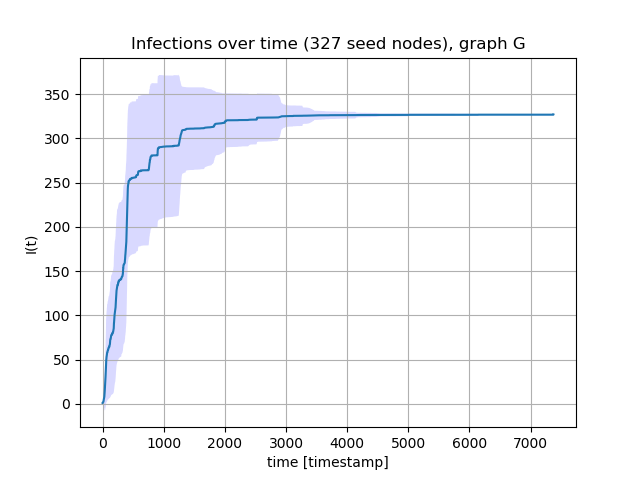
\includegraphics[width=\textwidth]{img/infections_G.png}
        \caption{Graph \(G\)}
	    \label{fig:infections_over_time_G}
    \end{subfigure}
%    ~ % spacing
    \begin{subfigure}[b]{0.32\textwidth}
        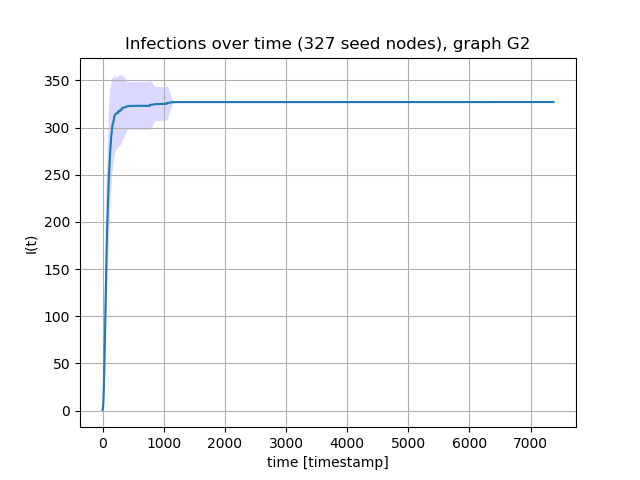
\includegraphics[width=\textwidth]{img/infections_G2.png}
        \caption{Graph \(G_2\)}
	    \label{fig:infections_over_time_G2}
    \end{subfigure}
%     ~ % spacing
    \begin{subfigure}[b]{0.32\textwidth}
        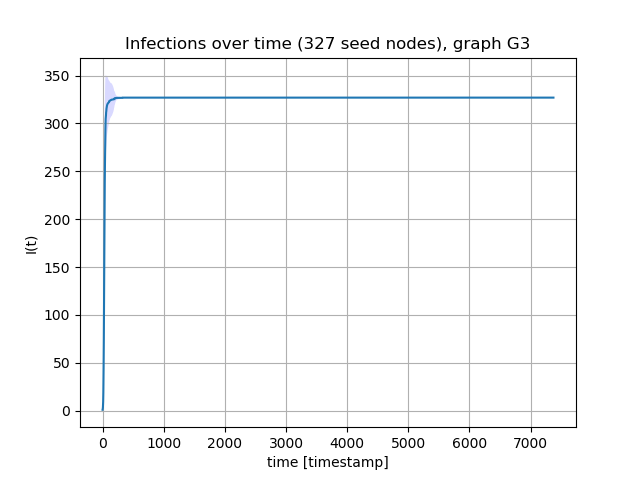
\includegraphics[width=\textwidth]{img/infections_G3.png}
        \caption{Graph \(G_3\)}
	    \label{fig:infections_over_time_G3}
    \end{subfigure}
    \caption{The average number of infected nodes as a function of the time step, $\mathrm{E}[I(t)]$ on several temporal graphs. The standard deviation, $\sqrt{\mathrm{Var}{[I(t)}]}$ is indicated by the shaded area.}
    \label{fig:infections_over_time}

    \centering
    \begin{subfigure}[b]{0.32\textwidth}
        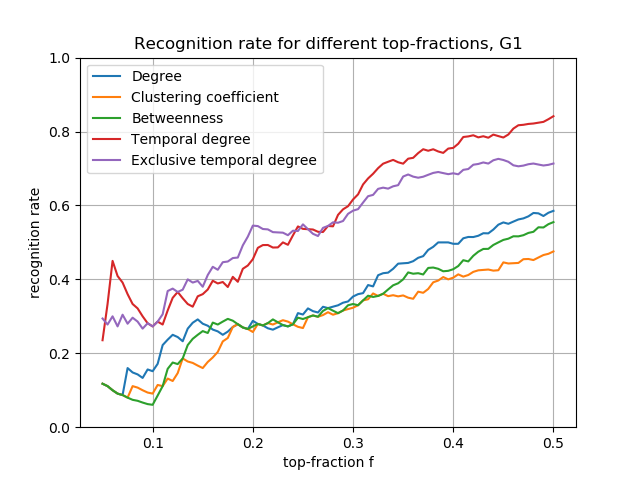
\includegraphics[width=\textwidth]{img/rankG.png}
        \caption{Graph \(G\)}
	    \label{fig:recognition_rates_G}
    \end{subfigure}
%    ~ % spacing
    \begin{subfigure}[b]{0.32\textwidth}
        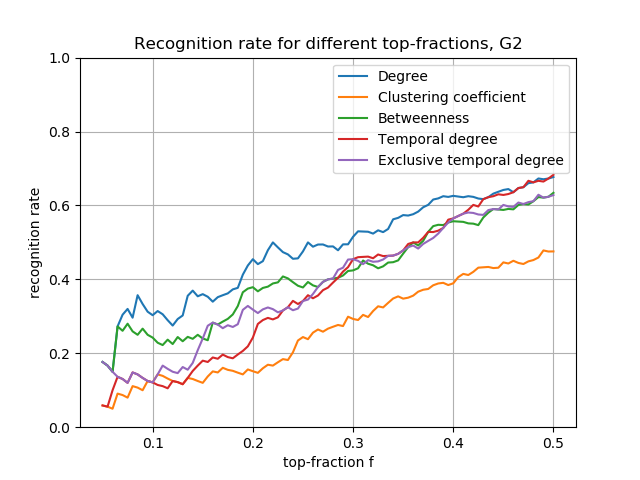
\includegraphics[width=\textwidth]{img/rankG2.png}
        \caption{Graph \(G_2\)}
	    \label{fig:recognition_rates_G2}
    \end{subfigure}
%     ~ % spacing
    \begin{subfigure}[b]{0.32\textwidth}
        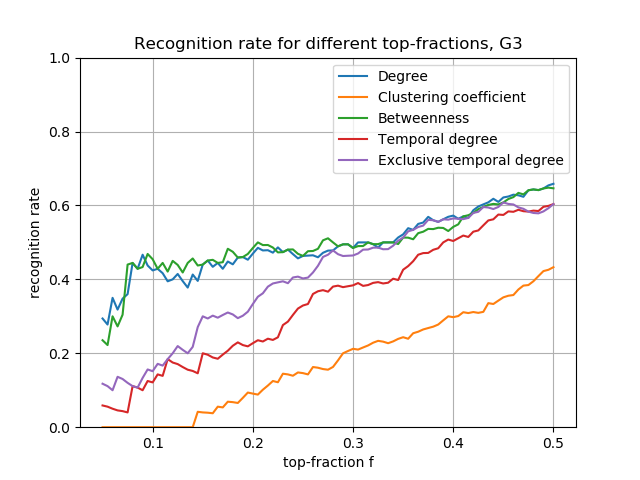
\includegraphics[width=\textwidth]{img/rankG3.png}
        \caption{Graph \(G_3\)}
	    \label{fig:recognition_rates_G3}
    \end{subfigure}
    \caption{Degree distribution of nodes in the aggregated graph.}
    \label{fig:recognition_rates}

    \centering
    \begin{subfigure}[b]{0.32\textwidth}
        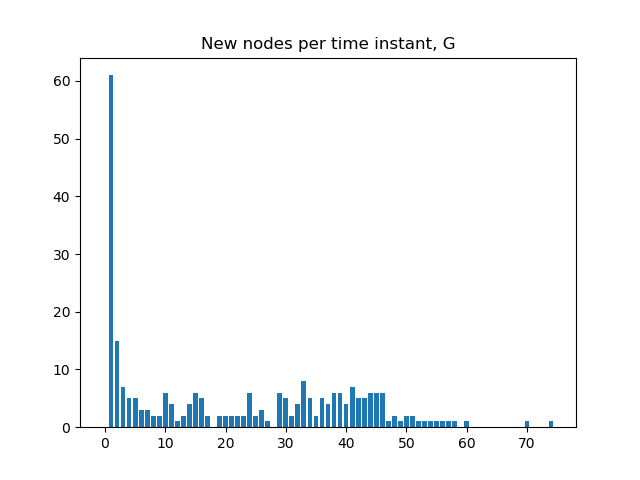
\includegraphics[width=\textwidth]{img/newNodesG.png}
        \caption{Graph \(G\)}
	    \label{fig:degree_distribution_G}
    \end{subfigure}
%    ~ % spacing
    \begin{subfigure}[b]{0.32\textwidth}
        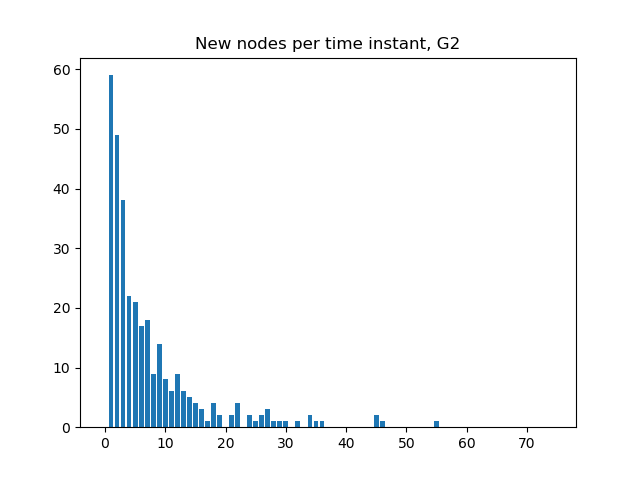
\includegraphics[width=\textwidth]{img/newNodesG2.png}
        \caption{Graph \(G_2\)}
	    \label{fig:degree_distribution_G2}
    \end{subfigure}
%     ~ % spacing
    \begin{subfigure}[b]{0.32\textwidth}
        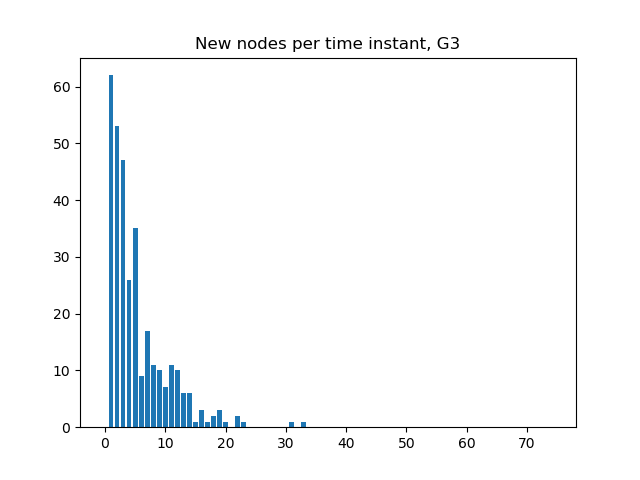
\includegraphics[width=\textwidth]{img/newNodesG3.png}
        \caption{Graph \(G_3\)}
	    \label{fig:degree_distribution_G3}
    \end{subfigure}
    \caption{Degree distribution of nodes in several graphs. \(G\) is the aggregated graph from the dataset (see part~\ref{sec:partA}), \(G_2\) is \(G\) but with the timestamps of edges shuffled and \(G_3\) is \(G\) but with the timestamps randomly redistributed across the edges. For details, see part~\ref{sec:partC}.}
    \label{fig:degree_distribution}
\end{figure}

newNodesG


\subsection*{Conclusion}
\todo{}




\end{document}
